% Created by tikzDevice version 0.12.6 on 2026-03-17 20:29:27
% !TEX encoding = UTF-8 Unicode
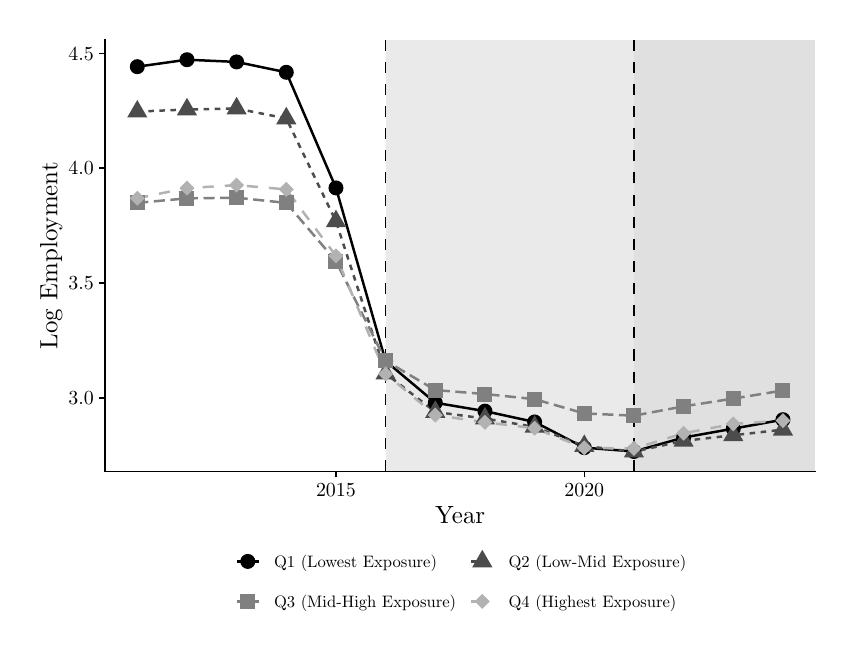
\begin{tikzpicture}[x=1pt,y=1pt]
\definecolor{fillColor}{RGB}{255,255,255}
\path[use as bounding box,fill=fillColor,fill opacity=0.00] (0,0) rectangle (289.08,216.81);
\begin{scope}
\path[clip] (  0.00,  0.00) rectangle (289.08,216.81);
\definecolor{drawColor}{RGB}{255,255,255}
\definecolor{fillColor}{RGB}{255,255,255}

\path[draw=drawColor,line width= 0.5pt,line join=round,line cap=round,fill=fillColor] (  0.00,  0.00) rectangle (289.08,216.81);
\end{scope}
\begin{scope}
\path[clip] ( 27.95, 56.52) rectangle (284.58,212.31);
\definecolor{fillColor}{RGB}{255,255,255}

\path[fill=fillColor] ( 27.95, 56.52) rectangle (284.58,212.31);
\definecolor{fillColor}{RGB}{153,153,153}

\path[fill=fillColor,fill opacity=0.20] (129.34, 56.52) rectangle (219.08,212.31);
\definecolor{fillColor}{RGB}{102,102,102}

\path[fill=fillColor,fill opacity=0.20] (219.08, 56.52) rectangle (284.58,212.31);
\definecolor{drawColor}{RGB}{0,0,0}

\path[draw=drawColor,line width= 0.6pt,dash pattern=on 4pt off 4pt ,line join=round] (129.34, 56.52) -- (129.34,212.31);

\path[draw=drawColor,line width= 0.6pt,dash pattern=on 4pt off 4pt ,line join=round] (219.08, 56.52) -- (219.08,212.31);

\path[draw=drawColor,line width= 0.9pt,line join=round] ( 39.61,202.71) --
	( 57.56,205.23) --
	( 75.50,204.43) --
	( 93.45,200.68) --
	(111.40,158.90) --
	(129.34, 96.35) --
	(147.29, 81.28) --
	(165.24, 78.24) --
	(183.18, 74.33) --
	(201.13, 65.05) --
	(219.08, 63.66) --
	(237.02, 68.70) --
	(254.97, 71.92) --
	(272.91, 75.16);
\definecolor{drawColor}{gray}{0.30}

\path[draw=drawColor,line width= 0.9pt,dash pattern=on 2pt off 2pt ,line join=round] ( 39.61,186.47) --
	( 57.56,187.25) --
	( 75.50,187.59) --
	( 93.45,184.01) --
	(111.40,146.83) --
	(129.34, 91.85) --
	(147.29, 77.96) --
	(165.24, 75.56) --
	(183.18, 72.54) --
	(201.13, 65.63) --
	(219.08, 63.60) --
	(237.02, 67.50) --
	(254.97, 69.53) --
	(272.91, 71.55);
\definecolor{drawColor}{gray}{0.50}

\path[draw=drawColor,line width= 0.9pt,dash pattern=on 4pt off 2pt ,line join=round] ( 39.61,153.50) --
	( 57.56,155.13) --
	( 75.50,155.37) --
	( 93.45,153.49) --
	(111.40,132.45) --
	(129.34, 96.45) --
	(147.29, 85.86) --
	(165.24, 84.43) --
	(183.18, 82.57) --
	(201.13, 77.41) --
	(219.08, 76.61) --
	(237.02, 79.97) --
	(254.97, 82.78) --
	(272.91, 85.70);
\definecolor{drawColor}{gray}{0.70}

\path[draw=drawColor,line width= 0.9pt,dash pattern=on 4pt off 4pt ,line join=round] ( 39.61,155.18) --
	( 57.56,158.85) --
	( 75.50,159.91) --
	( 93.45,158.37) --
	(111.40,134.34) --
	(129.34, 91.68) --
	(147.29, 76.80) --
	(165.24, 74.22) --
	(183.18, 72.07) --
	(201.13, 64.94) --
	(219.08, 64.74) --
	(237.02, 70.24) --
	(254.97, 73.64) --
	(272.91, 74.83);
\definecolor{fillColor}{RGB}{0,0,0}

\path[fill=fillColor] ( 39.61,202.71) circle (  2.71);
\definecolor{fillColor}{gray}{0.30}

\path[fill=fillColor] ( 39.61,190.69) --
	( 43.26,184.37) --
	( 35.96,184.37) --
	cycle;
\definecolor{fillColor}{gray}{0.50}

\path[fill=fillColor] ( 36.90,150.79) --
	( 42.32,150.79) --
	( 42.32,156.21) --
	( 36.90,156.21) --
	cycle;
\definecolor{fillColor}{gray}{0.70}

\path[fill=fillColor] ( 36.90,155.18) --
	( 39.61,157.89) --
	( 42.32,155.18) --
	( 39.61,152.47) --
	cycle;
\definecolor{fillColor}{RGB}{0,0,0}

\path[fill=fillColor] ( 57.56,205.23) circle (  2.71);
\definecolor{fillColor}{gray}{0.30}

\path[fill=fillColor] ( 57.56,191.47) --
	( 61.21,185.14) --
	( 53.91,185.14) --
	cycle;
\definecolor{fillColor}{gray}{0.50}

\path[fill=fillColor] ( 54.85,152.42) --
	( 60.27,152.42) --
	( 60.27,157.84) --
	( 54.85,157.84) --
	cycle;
\definecolor{fillColor}{gray}{0.70}

\path[fill=fillColor] ( 54.85,158.85) --
	( 57.56,161.56) --
	( 60.27,158.85) --
	( 57.56,156.14) --
	cycle;
\definecolor{fillColor}{RGB}{0,0,0}

\path[fill=fillColor] ( 75.50,204.43) circle (  2.71);
\definecolor{fillColor}{gray}{0.30}

\path[fill=fillColor] ( 75.50,191.81) --
	( 79.15,185.49) --
	( 71.85,185.49) --
	cycle;
\definecolor{fillColor}{gray}{0.50}

\path[fill=fillColor] ( 72.79,152.66) --
	( 78.21,152.66) --
	( 78.21,158.08) --
	( 72.79,158.08) --
	cycle;
\definecolor{fillColor}{gray}{0.70}

\path[fill=fillColor] ( 72.79,159.91) --
	( 75.50,162.62) --
	( 78.21,159.91) --
	( 75.50,157.20) --
	cycle;
\definecolor{fillColor}{RGB}{0,0,0}

\path[fill=fillColor] ( 93.45,200.68) circle (  2.71);
\definecolor{fillColor}{gray}{0.30}

\path[fill=fillColor] ( 93.45,188.23) --
	( 97.10,181.90) --
	( 89.80,181.90) --
	cycle;
\definecolor{fillColor}{gray}{0.50}

\path[fill=fillColor] ( 90.74,150.78) --
	( 96.16,150.78) --
	( 96.16,156.20) --
	( 90.74,156.20) --
	cycle;
\definecolor{fillColor}{gray}{0.70}

\path[fill=fillColor] ( 90.74,158.37) --
	( 93.45,161.08) --
	( 96.16,158.37) --
	( 93.45,155.66) --
	cycle;
\definecolor{fillColor}{RGB}{0,0,0}

\path[fill=fillColor] (111.40,158.90) circle (  2.71);
\definecolor{fillColor}{gray}{0.30}

\path[fill=fillColor] (111.40,151.05) --
	(115.05,144.72) --
	(107.75,144.72) --
	cycle;
\definecolor{fillColor}{gray}{0.50}

\path[fill=fillColor] (108.69,129.74) --
	(114.11,129.74) --
	(114.11,135.16) --
	(108.69,135.16) --
	cycle;
\definecolor{fillColor}{gray}{0.70}

\path[fill=fillColor] (108.69,134.34) --
	(111.40,137.06) --
	(114.11,134.34) --
	(111.40,131.63) --
	cycle;
\definecolor{fillColor}{RGB}{0,0,0}

\path[fill=fillColor] (129.34, 96.35) circle (  2.71);
\definecolor{fillColor}{gray}{0.30}

\path[fill=fillColor] (129.34, 96.06) --
	(132.99, 89.74) --
	(125.69, 89.74) --
	cycle;
\definecolor{fillColor}{gray}{0.50}

\path[fill=fillColor] (126.63, 93.74) --
	(132.05, 93.74) --
	(132.05, 99.16) --
	(126.63, 99.16) --
	cycle;
\definecolor{fillColor}{gray}{0.70}

\path[fill=fillColor] (126.63, 91.68) --
	(129.34, 94.39) --
	(132.05, 91.68) --
	(129.34, 88.96) --
	cycle;
\definecolor{fillColor}{RGB}{0,0,0}

\path[fill=fillColor] (147.29, 81.28) circle (  2.71);
\definecolor{fillColor}{gray}{0.30}

\path[fill=fillColor] (147.29, 82.17) --
	(150.94, 75.85) --
	(143.64, 75.85) --
	cycle;
\definecolor{fillColor}{gray}{0.50}

\path[fill=fillColor] (144.58, 83.15) --
	(150.00, 83.15) --
	(150.00, 88.57) --
	(144.58, 88.57) --
	cycle;
\definecolor{fillColor}{gray}{0.70}

\path[fill=fillColor] (144.58, 76.80) --
	(147.29, 79.51) --
	(150.00, 76.80) --
	(147.29, 74.09) --
	cycle;
\definecolor{fillColor}{RGB}{0,0,0}

\path[fill=fillColor] (165.24, 78.24) circle (  2.71);
\definecolor{fillColor}{gray}{0.30}

\path[fill=fillColor] (165.24, 79.78) --
	(168.89, 73.45) --
	(161.58, 73.45) --
	cycle;
\definecolor{fillColor}{gray}{0.50}

\path[fill=fillColor] (162.53, 81.72) --
	(167.95, 81.72) --
	(167.95, 87.14) --
	(162.53, 87.14) --
	cycle;
\definecolor{fillColor}{gray}{0.70}

\path[fill=fillColor] (162.53, 74.22) --
	(165.24, 76.93) --
	(167.95, 74.22) --
	(165.24, 71.50) --
	cycle;
\definecolor{fillColor}{RGB}{0,0,0}

\path[fill=fillColor] (183.18, 74.33) circle (  2.71);
\definecolor{fillColor}{gray}{0.30}

\path[fill=fillColor] (183.18, 76.76) --
	(186.83, 70.44) --
	(179.53, 70.44) --
	cycle;
\definecolor{fillColor}{gray}{0.50}

\path[fill=fillColor] (180.47, 79.86) --
	(185.89, 79.86) --
	(185.89, 85.28) --
	(180.47, 85.28) --
	cycle;
\definecolor{fillColor}{gray}{0.70}

\path[fill=fillColor] (180.47, 72.07) --
	(183.18, 74.78) --
	(185.89, 72.07) --
	(183.18, 69.36) --
	cycle;
\definecolor{fillColor}{RGB}{0,0,0}

\path[fill=fillColor] (201.13, 65.05) circle (  2.71);
\definecolor{fillColor}{gray}{0.30}

\path[fill=fillColor] (201.13, 69.84) --
	(204.78, 63.52) --
	(197.48, 63.52) --
	cycle;
\definecolor{fillColor}{gray}{0.50}

\path[fill=fillColor] (198.42, 74.70) --
	(203.84, 74.70) --
	(203.84, 80.13) --
	(198.42, 80.13) --
	cycle;
\definecolor{fillColor}{gray}{0.70}

\path[fill=fillColor] (198.42, 64.94) --
	(201.13, 67.65) --
	(203.84, 64.94) --
	(201.13, 62.23) --
	cycle;
\definecolor{fillColor}{RGB}{0,0,0}

\path[fill=fillColor] (219.08, 63.66) circle (  2.71);
\definecolor{fillColor}{gray}{0.30}

\path[fill=fillColor] (219.08, 67.82) --
	(222.73, 61.50) --
	(215.42, 61.50) --
	cycle;
\definecolor{fillColor}{gray}{0.50}

\path[fill=fillColor] (216.36, 73.90) --
	(221.79, 73.90) --
	(221.79, 79.32) --
	(216.36, 79.32) --
	cycle;
\definecolor{fillColor}{gray}{0.70}

\path[fill=fillColor] (216.36, 64.74) --
	(219.08, 67.45) --
	(221.79, 64.74) --
	(219.08, 62.03) --
	cycle;
\definecolor{fillColor}{RGB}{0,0,0}

\path[fill=fillColor] (237.02, 68.70) circle (  2.71);
\definecolor{fillColor}{gray}{0.30}

\path[fill=fillColor] (237.02, 71.71) --
	(240.67, 65.39) --
	(233.37, 65.39) --
	cycle;
\definecolor{fillColor}{gray}{0.50}

\path[fill=fillColor] (234.31, 77.26) --
	(239.73, 77.26) --
	(239.73, 82.68) --
	(234.31, 82.68) --
	cycle;
\definecolor{fillColor}{gray}{0.70}

\path[fill=fillColor] (234.31, 70.24) --
	(237.02, 72.95) --
	(239.73, 70.24) --
	(237.02, 67.53) --
	cycle;
\definecolor{fillColor}{RGB}{0,0,0}

\path[fill=fillColor] (254.97, 71.92) circle (  2.71);
\definecolor{fillColor}{gray}{0.30}

\path[fill=fillColor] (254.97, 73.75) --
	(258.62, 67.43) --
	(251.32, 67.43) --
	cycle;
\definecolor{fillColor}{gray}{0.50}

\path[fill=fillColor] (252.26, 80.07) --
	(257.68, 80.07) --
	(257.68, 85.49) --
	(252.26, 85.49) --
	cycle;
\definecolor{fillColor}{gray}{0.70}

\path[fill=fillColor] (252.26, 73.64) --
	(254.97, 76.35) --
	(257.68, 73.64) --
	(254.97, 70.93) --
	cycle;
\definecolor{fillColor}{RGB}{0,0,0}

\path[fill=fillColor] (272.91, 75.16) circle (  2.71);
\definecolor{fillColor}{gray}{0.30}

\path[fill=fillColor] (272.91, 75.76) --
	(276.57, 69.44) --
	(269.26, 69.44) --
	cycle;
\definecolor{fillColor}{gray}{0.50}

\path[fill=fillColor] (270.20, 82.99) --
	(275.63, 82.99) --
	(275.63, 88.41) --
	(270.20, 88.41) --
	cycle;
\definecolor{fillColor}{gray}{0.70}

\path[fill=fillColor] (270.20, 74.83) --
	(272.91, 77.54) --
	(275.63, 74.83) --
	(272.91, 72.12) --
	cycle;
\end{scope}
\begin{scope}
\path[clip] (  0.00,  0.00) rectangle (289.08,216.81);
\definecolor{drawColor}{RGB}{0,0,0}

\path[draw=drawColor,line width= 0.5pt,line join=round,line cap=rect] ( 27.95, 56.52) --
	( 27.95,212.31);
\end{scope}
\begin{scope}
\path[clip] (  0.00,  0.00) rectangle (289.08,216.81);
\definecolor{drawColor}{RGB}{0,0,0}

\node[text=drawColor,anchor=base east,inner sep=0pt, outer sep=0pt, scale=  0.72] at ( 23.90, 80.58) {3.0};

\node[text=drawColor,anchor=base east,inner sep=0pt, outer sep=0pt, scale=  0.72] at ( 23.90,122.08) {3.5};

\node[text=drawColor,anchor=base east,inner sep=0pt, outer sep=0pt, scale=  0.72] at ( 23.90,163.58) {4.0};

\node[text=drawColor,anchor=base east,inner sep=0pt, outer sep=0pt, scale=  0.72] at ( 23.90,205.08) {4.5};
\end{scope}
\begin{scope}
\path[clip] (  0.00,  0.00) rectangle (289.08,216.81);
\definecolor{drawColor}{RGB}{0,0,0}

\path[draw=drawColor,line width= 0.5pt,line join=round] ( 25.70, 83.06) --
	( 27.95, 83.06);

\path[draw=drawColor,line width= 0.5pt,line join=round] ( 25.70,124.56) --
	( 27.95,124.56);

\path[draw=drawColor,line width= 0.5pt,line join=round] ( 25.70,166.06) --
	( 27.95,166.06);

\path[draw=drawColor,line width= 0.5pt,line join=round] ( 25.70,207.56) --
	( 27.95,207.56);
\end{scope}
\begin{scope}
\path[clip] (  0.00,  0.00) rectangle (289.08,216.81);
\definecolor{drawColor}{RGB}{0,0,0}

\path[draw=drawColor,line width= 0.5pt,line join=round,line cap=rect] ( 27.95, 56.52) --
	(284.58, 56.52);
\end{scope}
\begin{scope}
\path[clip] (  0.00,  0.00) rectangle (289.08,216.81);
\definecolor{drawColor}{RGB}{0,0,0}

\path[draw=drawColor,line width= 0.5pt,line join=round] (111.40, 54.27) --
	(111.40, 56.52);

\path[draw=drawColor,line width= 0.5pt,line join=round] (201.13, 54.27) --
	(201.13, 56.52);
\end{scope}
\begin{scope}
\path[clip] (  0.00,  0.00) rectangle (289.08,216.81);
\definecolor{drawColor}{RGB}{0,0,0}

\node[text=drawColor,anchor=base,inner sep=0pt, outer sep=0pt, scale=  0.72] at (111.40, 47.51) {2015};

\node[text=drawColor,anchor=base,inner sep=0pt, outer sep=0pt, scale=  0.72] at (201.13, 47.51) {2020};
\end{scope}
\begin{scope}
\path[clip] (  0.00,  0.00) rectangle (289.08,216.81);
\definecolor{drawColor}{RGB}{0,0,0}

\node[text=drawColor,anchor=base,inner sep=0pt, outer sep=0pt, scale=  0.90] at (156.26, 37.67) {Year};
\end{scope}
\begin{scope}
\path[clip] (  0.00,  0.00) rectangle (289.08,216.81);
\definecolor{drawColor}{RGB}{0,0,0}

\node[text=drawColor,rotate= 90.00,anchor=base,inner sep=0pt, outer sep=0pt, scale=  0.90] at ( 10.70,134.42) {Log Employment};
\end{scope}
\begin{scope}
\path[clip] (  0.00,  0.00) rectangle (289.08,216.81);
\definecolor{drawColor}{RGB}{0,0,0}

\path[draw=drawColor,line width= 0.9pt,line join=round] ( 75.56, 23.94) -- ( 83.52, 23.94);
\definecolor{fillColor}{RGB}{0,0,0}

\path[fill=fillColor] ( 79.54, 23.94) circle (  2.71);
\end{scope}
\begin{scope}
\path[clip] (  0.00,  0.00) rectangle (289.08,216.81);
\definecolor{drawColor}{gray}{0.30}

\path[draw=drawColor,line width= 0.9pt,dash pattern=on 2pt off 2pt ,line join=round] (160.30, 23.94) -- (168.27, 23.94);
\definecolor{fillColor}{gray}{0.30}

\path[fill=fillColor] (164.28, 28.15) --
	(167.93, 21.83) --
	(160.63, 21.83) --
	cycle;
\end{scope}
\begin{scope}
\path[clip] (  0.00,  0.00) rectangle (289.08,216.81);
\definecolor{drawColor}{gray}{0.50}

\path[draw=drawColor,line width= 0.9pt,dash pattern=on 4pt off 2pt ,line join=round] ( 75.56,  9.48) -- ( 83.52,  9.48);
\definecolor{fillColor}{gray}{0.50}

\path[fill=fillColor] ( 76.83,  6.77) --
	( 82.25,  6.77) --
	( 82.25, 12.19) --
	( 76.83, 12.19) --
	cycle;
\end{scope}
\begin{scope}
\path[clip] (  0.00,  0.00) rectangle (289.08,216.81);
\definecolor{drawColor}{gray}{0.70}

\path[draw=drawColor,line width= 0.9pt,dash pattern=on 4pt off 4pt ,line join=round] (160.30,  9.48) -- (168.27,  9.48);
\definecolor{fillColor}{gray}{0.70}

\path[fill=fillColor] (161.57,  9.48) --
	(164.28, 12.19) --
	(166.99,  9.48) --
	(164.28,  6.77) --
	cycle;
\end{scope}
\begin{scope}
\path[clip] (  0.00,  0.00) rectangle (289.08,216.81);
\definecolor{drawColor}{RGB}{0,0,0}

\node[text=drawColor,anchor=base west,inner sep=0pt, outer sep=0pt, scale=  0.60] at ( 89.02, 21.87) {Q1 (Lowest Exposure)};
\end{scope}
\begin{scope}
\path[clip] (  0.00,  0.00) rectangle (289.08,216.81);
\definecolor{drawColor}{RGB}{0,0,0}

\node[text=drawColor,anchor=base west,inner sep=0pt, outer sep=0pt, scale=  0.60] at (173.76, 21.87) {Q2 (Low-Mid Exposure)};
\end{scope}
\begin{scope}
\path[clip] (  0.00,  0.00) rectangle (289.08,216.81);
\definecolor{drawColor}{RGB}{0,0,0}

\node[text=drawColor,anchor=base west,inner sep=0pt, outer sep=0pt, scale=  0.60] at ( 89.02,  7.41) {Q3 (Mid-High Exposure)};
\end{scope}
\begin{scope}
\path[clip] (  0.00,  0.00) rectangle (289.08,216.81);
\definecolor{drawColor}{RGB}{0,0,0}

\node[text=drawColor,anchor=base west,inner sep=0pt, outer sep=0pt, scale=  0.60] at (173.76,  7.41) {Q4 (Highest Exposure)};
\end{scope}
\end{tikzpicture}
